This chapter describes how the use of the different datasets were implemented and presented. The structure and functions are divided into the backend, which governs collection and manipulation of data, and the frontend which presents the data in a graphical user interface (GUI).

\section{The Backend}
The thesis is divided into two: The backend and the frontend. The backend is responsible for providing the frontend all the data and deeper functions it needs to visualize and administrate data to show in graphs. The backend is partitioned into modules based on each data source available. Each module may also be run individually for testing and easy viewing purposes. The twitter module is unique as it requires 4 application programming interface (API) keys to work properly. The instructions for this set-up is found in the README.md file in the twitter module's directory.







\subsection{The Norwegian Institute of Public Health}
There are two different sets of data, which is divided into separate modules, it was a simple job to plot them in a graph using pythons matplotlib library. Figure \ref{fig:infstat} show the three last seasons of influenza in regards to observed virus infections. The plotting was done manually as NPIH only provides the data in reports that are in pdf files on their official website\cite{fhi}.

\begin{figure}[h]
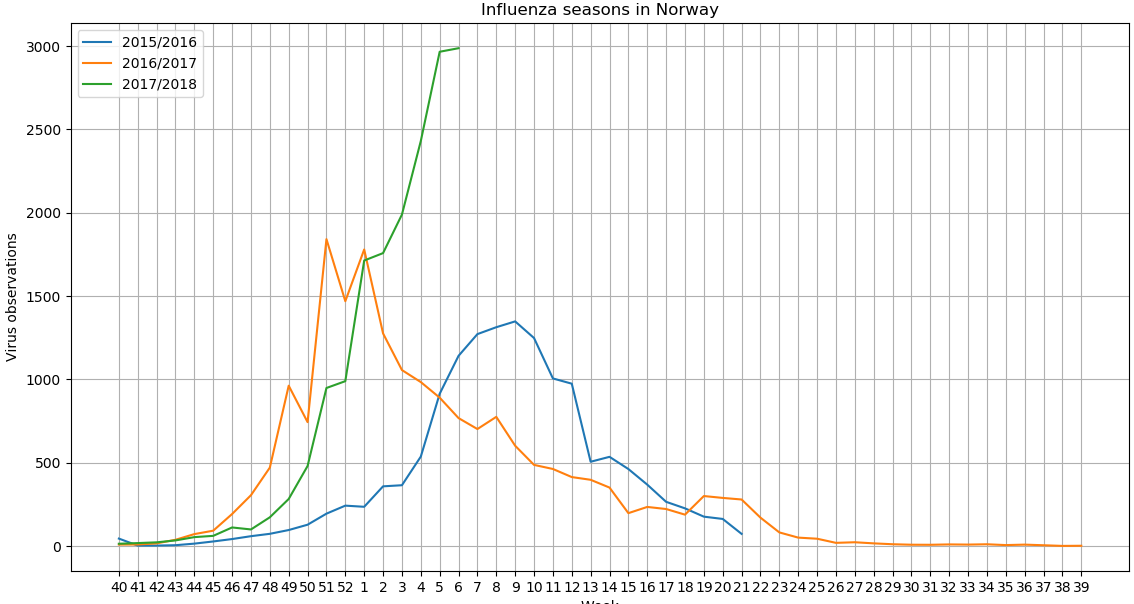
\includegraphics[width=16cm]{influenza_15_till_18}
\centering
\caption{Influenza virus observation}
\label{fig:infstat}
\end{figure}

Figure \ref{fig:ilsstat} shows the influenza-like illnesses (ILI) of the year 2016/2017. This was not done manually as data was provided in a simple .xlsx file which was read by python's openpyxl module, processed and then drawn as a graph.

\begin{figure}[ht]
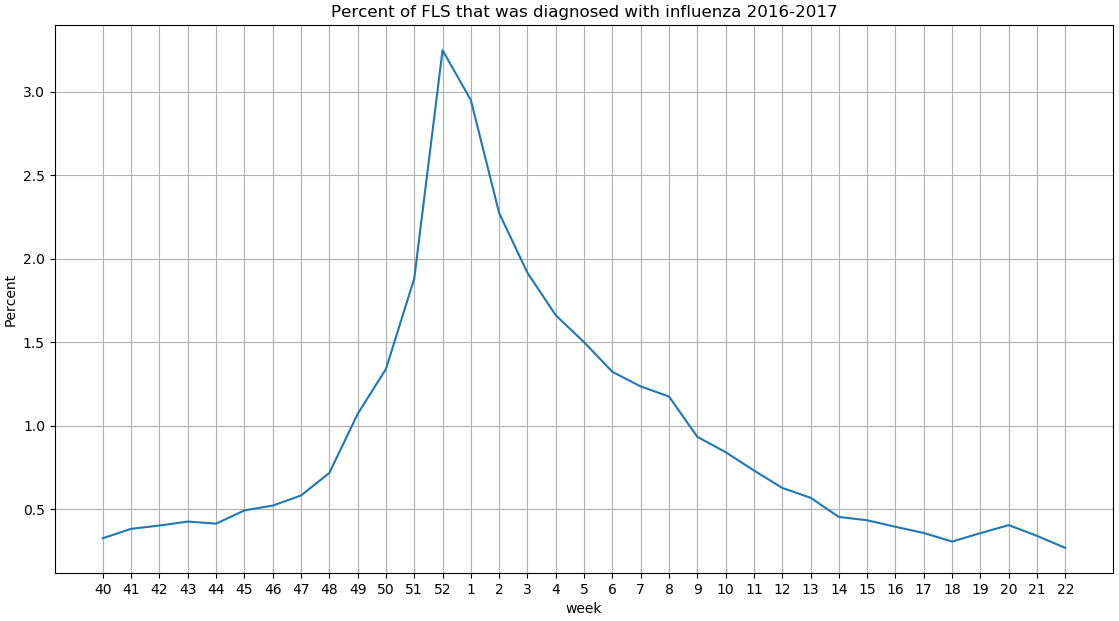
\includegraphics[width=16cm]{ILS_16_till_17}
\centering
\caption{Influenza-like illnesses season 2016/2017}
\label{fig:ilsstat}
\end{figure}

\newpage









\subsection{The Norwegian Public Roads Administration}
From the XML statistics, simple graphs were created in python showing the total annual traffic on Norwegian roads from 2002 to 2015 on a monthly basis as seen in figure \ref{fig:anualtotal}.

\begin{figure}[ht]
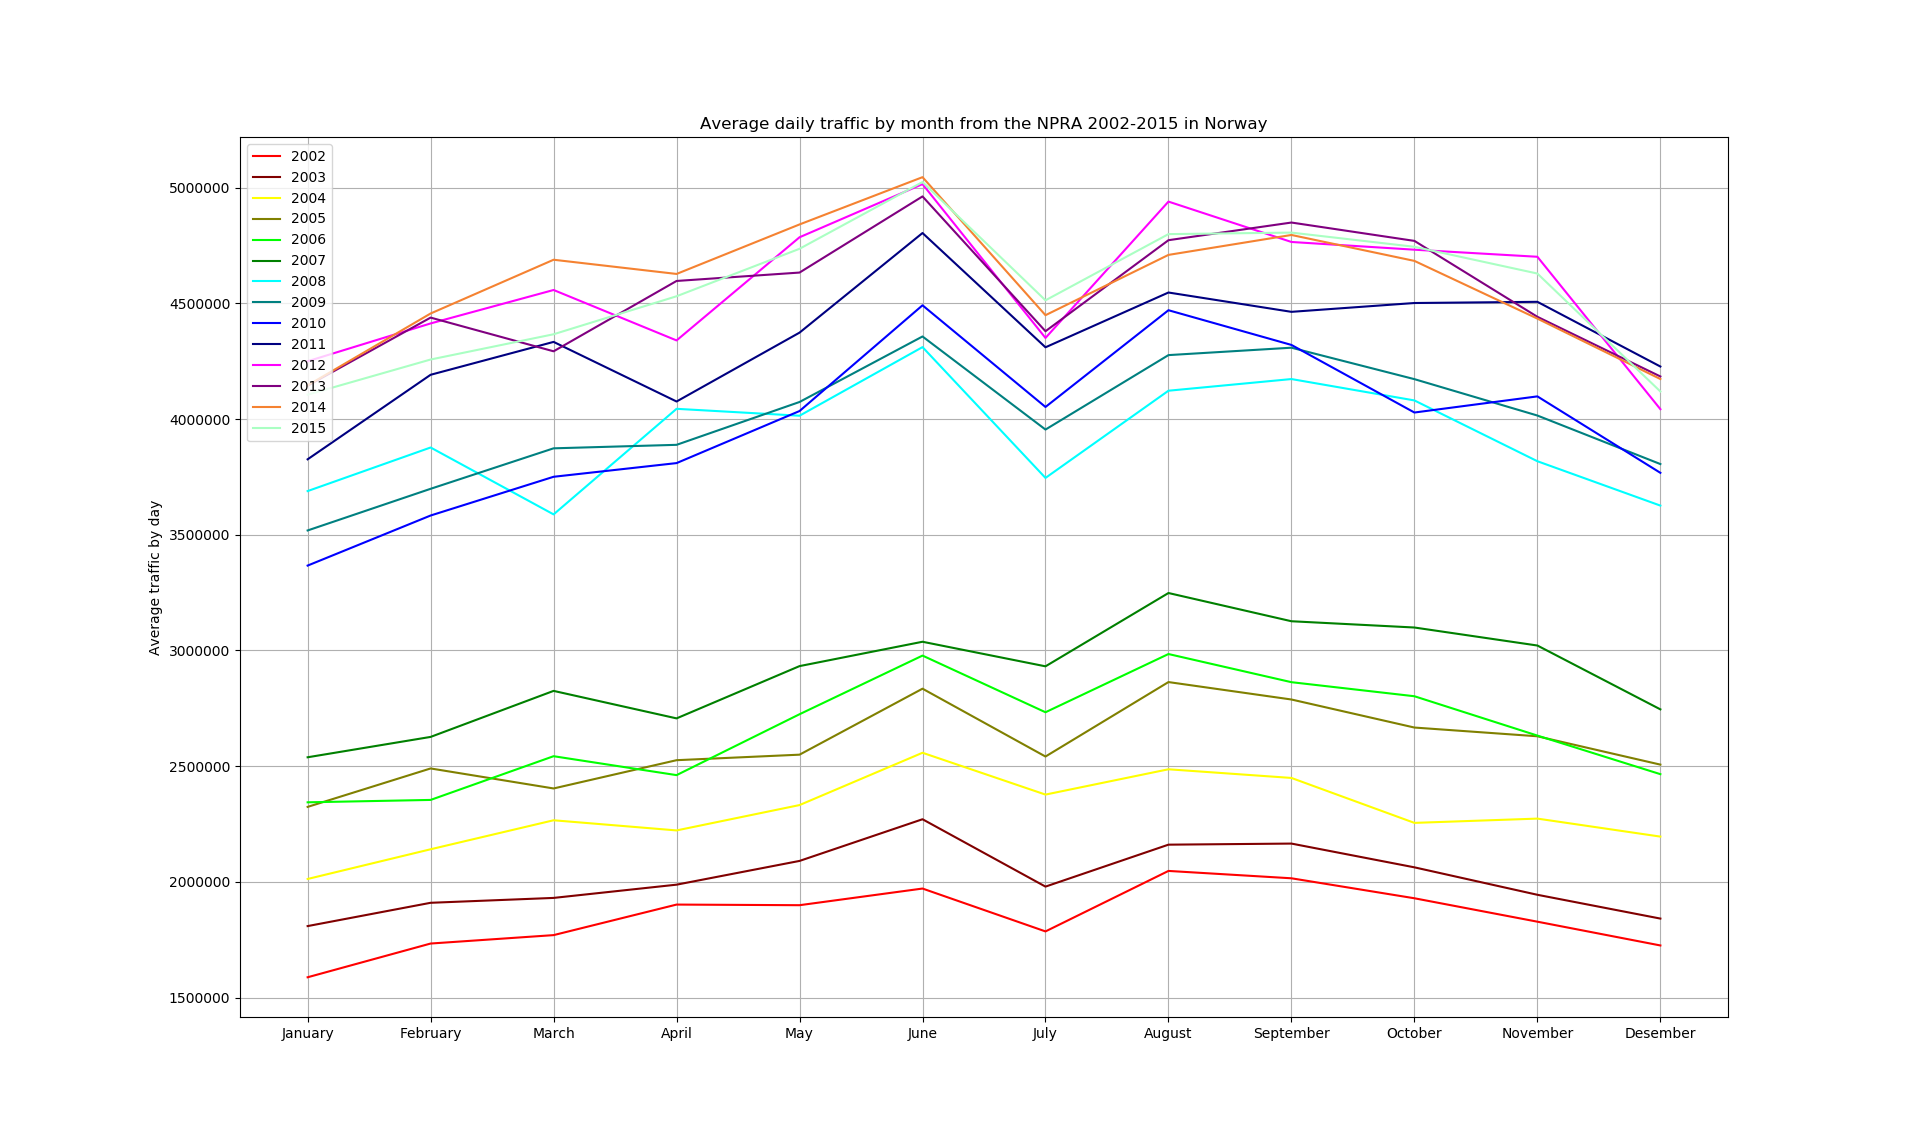
\includegraphics[width=16cm]{xml_02_15_annual_total}
\centering
\caption{Annual traffic 2002-2015}
\label{fig:anualtotal}
\end{figure}

Also derived from this dataset is the annual traffic of the two cities of Bergen and Oslo, which are cities of interest. Figure \ref{fig:anualbergen} shows the traffic in Bergen, and figure \ref{fig:anualoslo} show the traffic in Oslo.

\begin{figure}[ht]
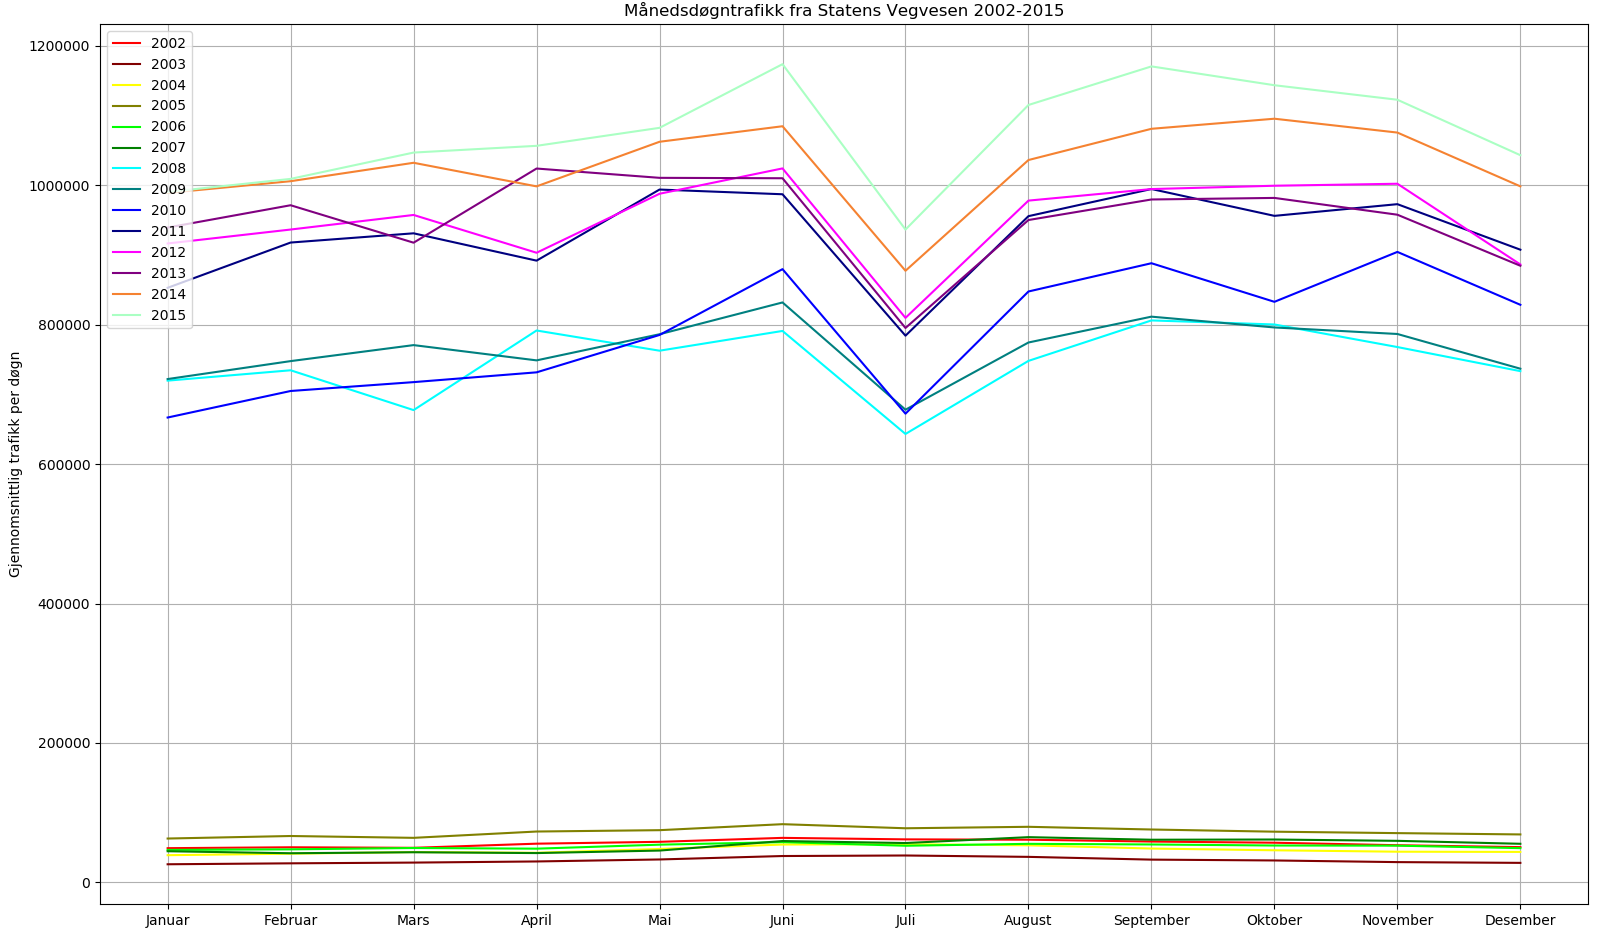
\includegraphics[width=16cm]{xml_02_15_annual_bergen}
\centering
\caption{Bergen traffic 2002-2015}
\label{fig:anualbergen}
\end{figure}

\begin{figure}[ht]
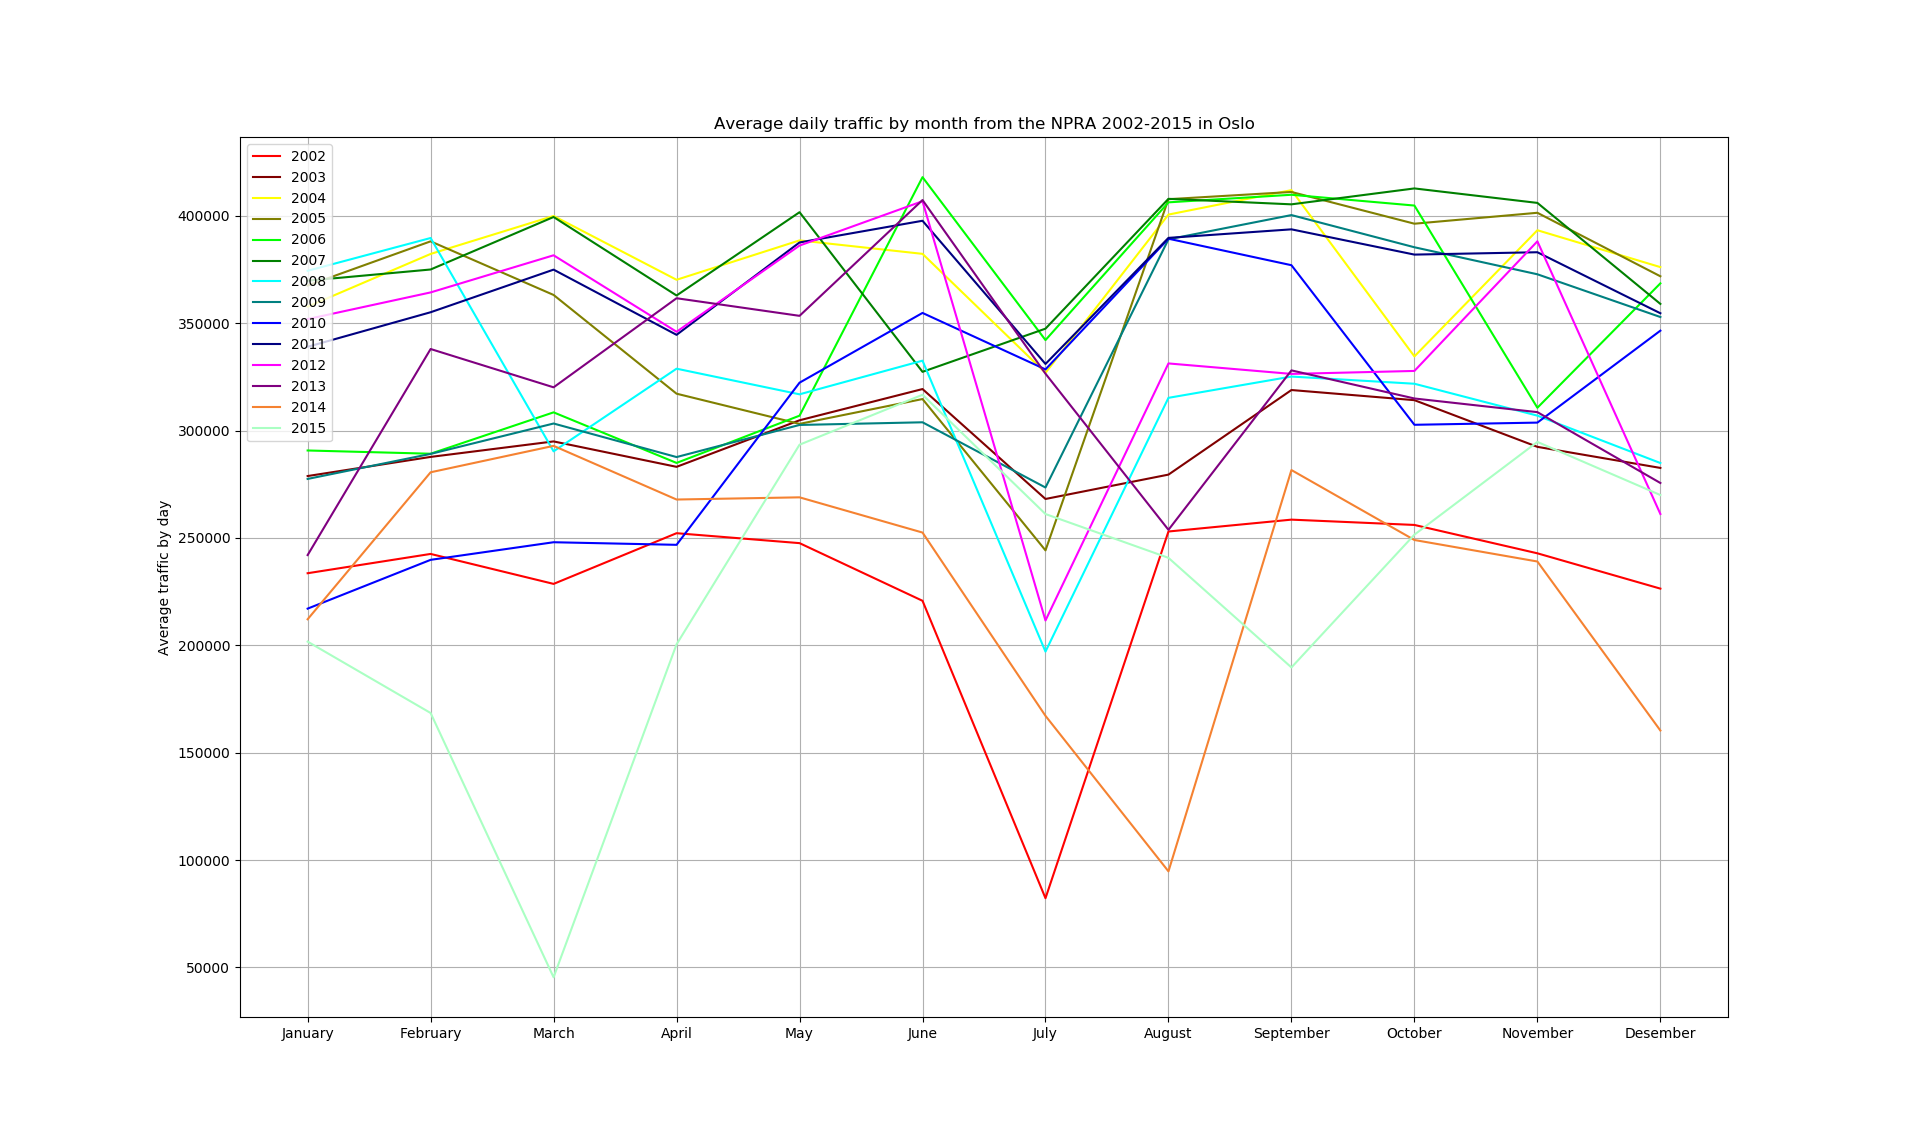
\includegraphics[width=16cm]{xml_02_15_annual_oslo}
\centering
\caption{Oslo traffic 2002-2015}
\label{fig:anualoslo}
\end{figure}
The dataset is in an XML file structure, a module named NPRA\_monthly.py was created that reads through all rows and collects the relevant columns into an array using Python's openpyxl module and then draws a graph using Python's matplotlib module. For the annual graph, every month of every year was collected. For the towns of Bergen and Oslo the correct roads were identified and then every year of every month of those roads was collected, loaded into an array and then drawn as a graph. The separate text files 'Bergen places.txt' and 'Oslo places.txt' is to make it easy to edit should these roads change in the future. This module when run individually accepts one argument from the user, either town of Oslo or Bergen may be provided to specify interest, if no argument is given the annual graph will show.

The problem of using these datasets is that the data is an average calculation of monthly traffic, this is too coarse for comparison against the influenza data as they are on a weekly basis. A set of traffic registration stations was needed to define the temporal bounds of each area of interest. Defined are the towns of Oslo, Stavanger, and Bergen, as well as the whole of Norway on a level 1 basis. The level 1 registrations are continuous throughout the year on an hourly basis and is exactly what this thesis requires. The module NPRA\_weekly.py captures these functions and also provides the user with command arguments if run individually. The commands are the cities of Bergen, Stavanger or Oslo if no commands are given the annual graph of the whole of Norway will be drawn instead.

Figures \ref{fig:weeklybergen}, \ref{fig:weeklyoslo} and \ref{fig:weeklystavanger} shows the traffic on a weekly basis. This provides a better resolution for better analysis.
\begin{figure}[ht]
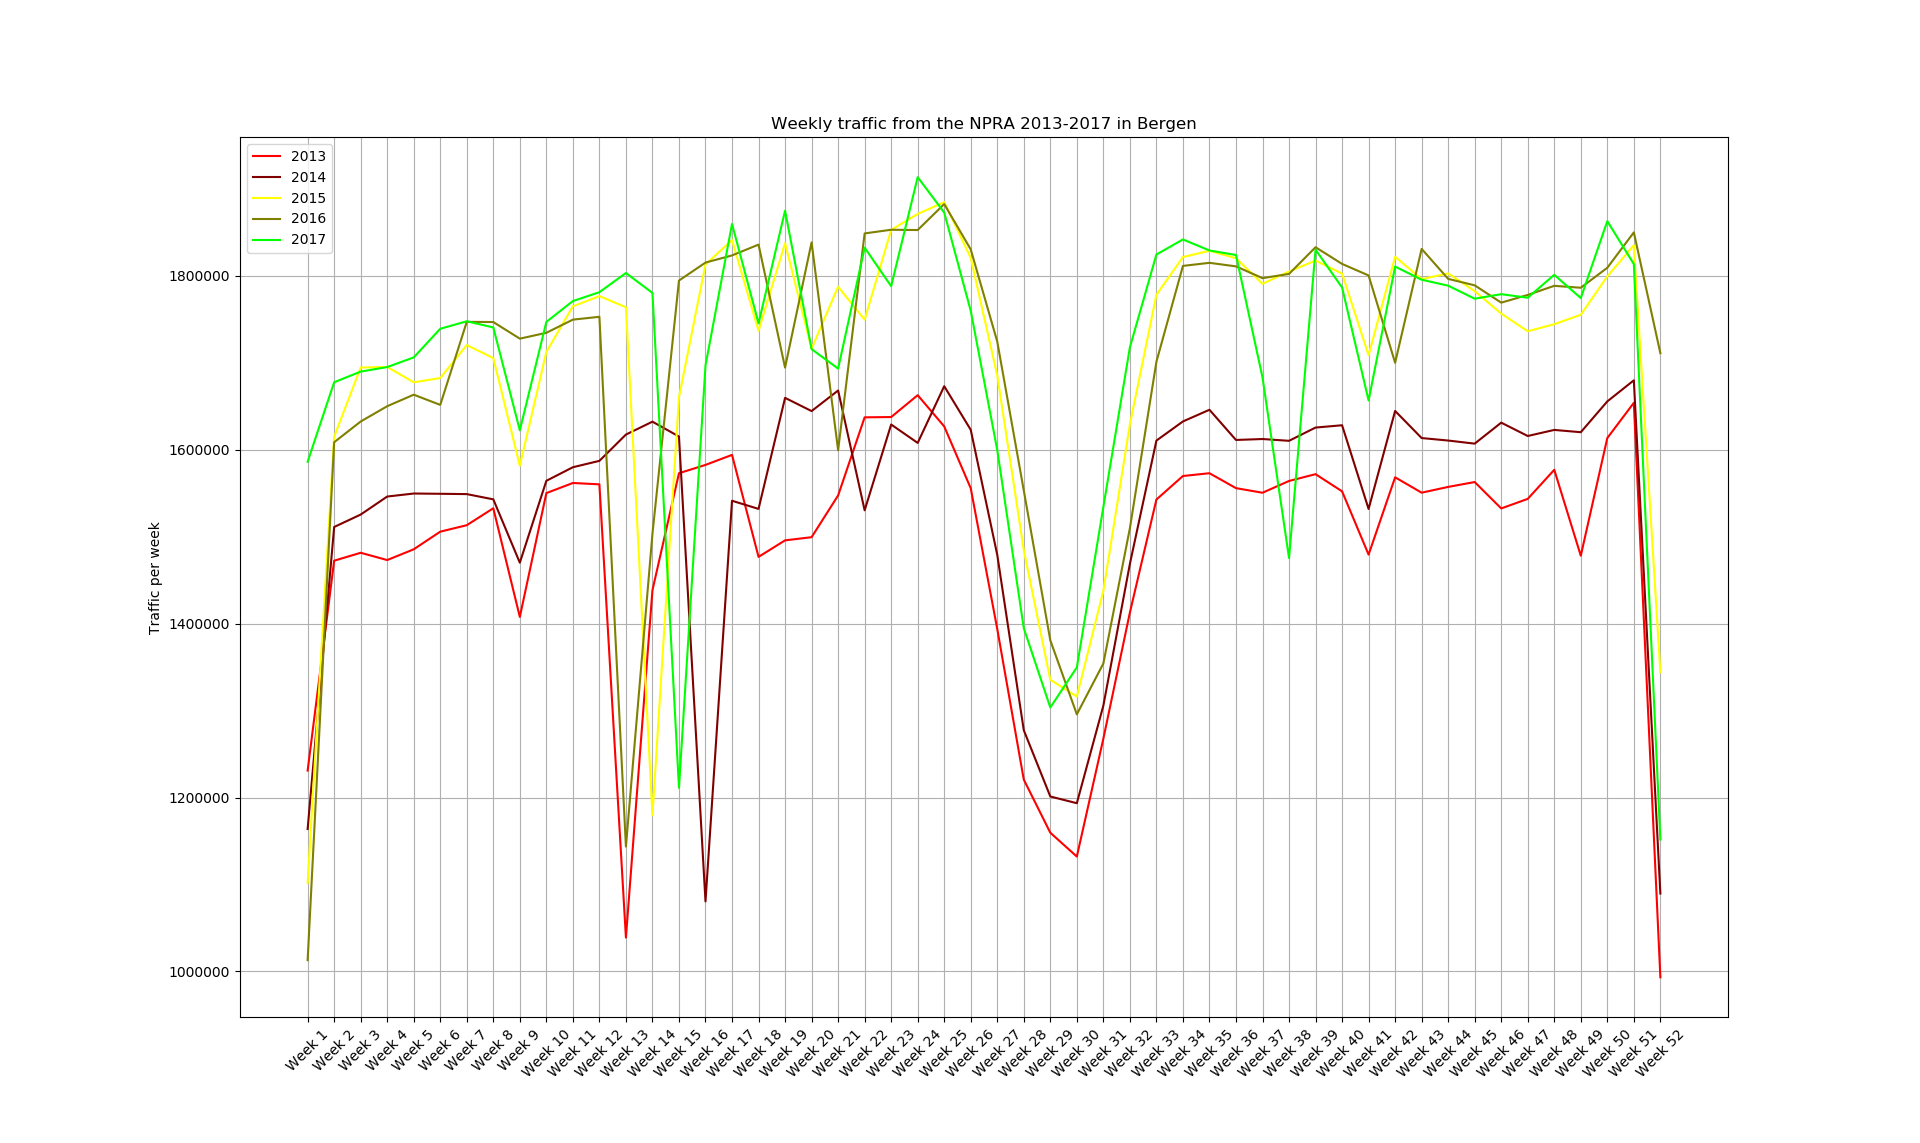
\includegraphics[width=16cm]{NPRA_13_17_weekly_bergen}
\centering
\caption{Weekly data of the city of Bergen}
\label{fig:weeklybergen}
\end{figure}

\begin{figure}[ht]
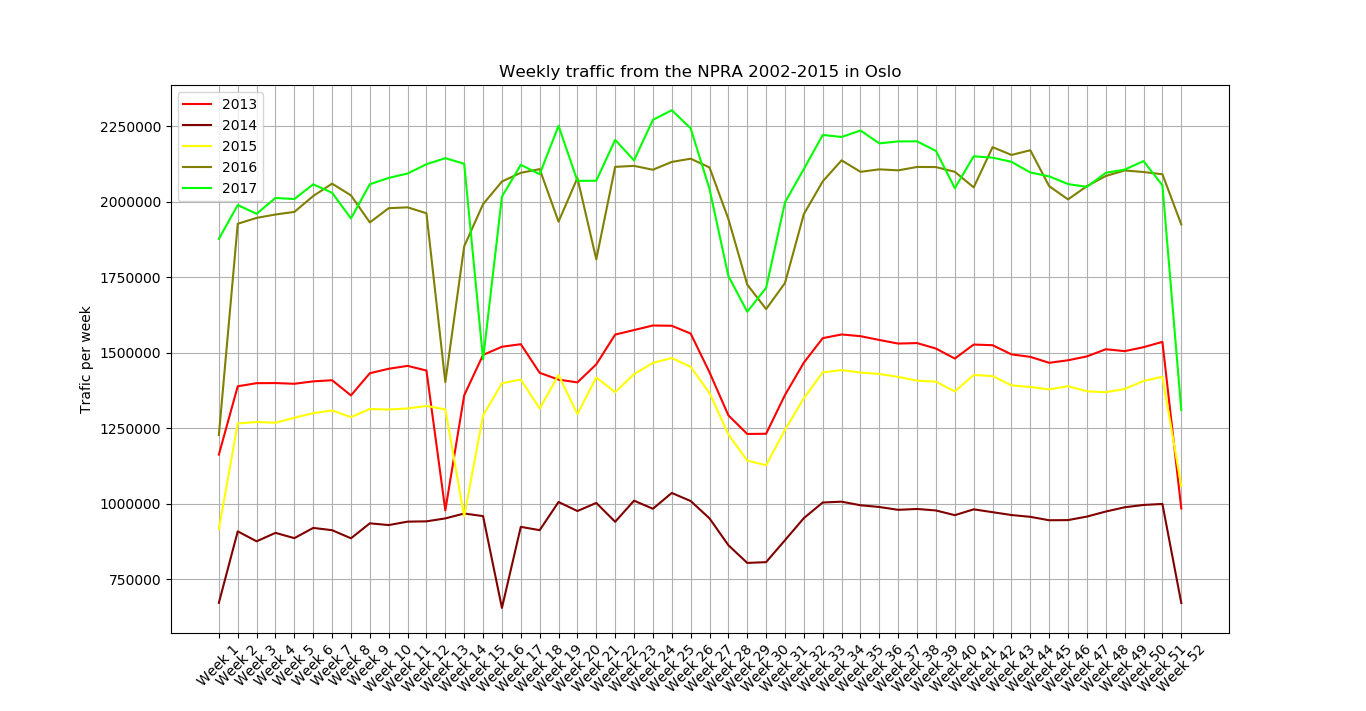
\includegraphics[width=16cm]{NPRA_13_17_weekly_oslo}
\centering
\caption{Weekly data of the city of Oslo}
\label{fig:weeklyoslo}
\end{figure}

\begin{figure}[ht]
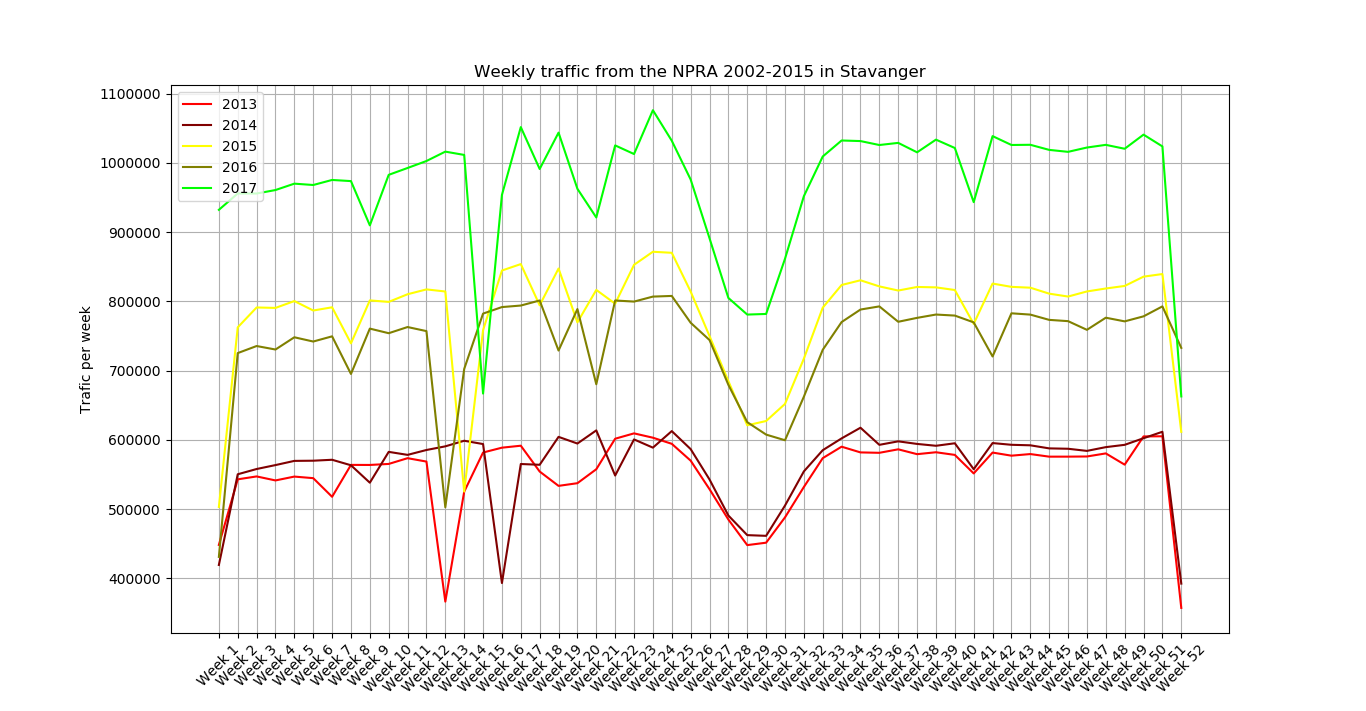
\includegraphics[width=16cm]{NPRA_13_17_weekly_stavanger}
\centering
\caption{Weekly data of the city of Stavanger}
\label{fig:weeklystavanger}
\end{figure}

Figure \ref{fig:boundsbergen}, \ref{fig:boundsoslo} and \ref{fig:boundsstavanger} shows the different geospatial bounds used to define the cities. The green circles with numbers inside show where and how many traffic registration stations there are.

\begin{figure}[ht]
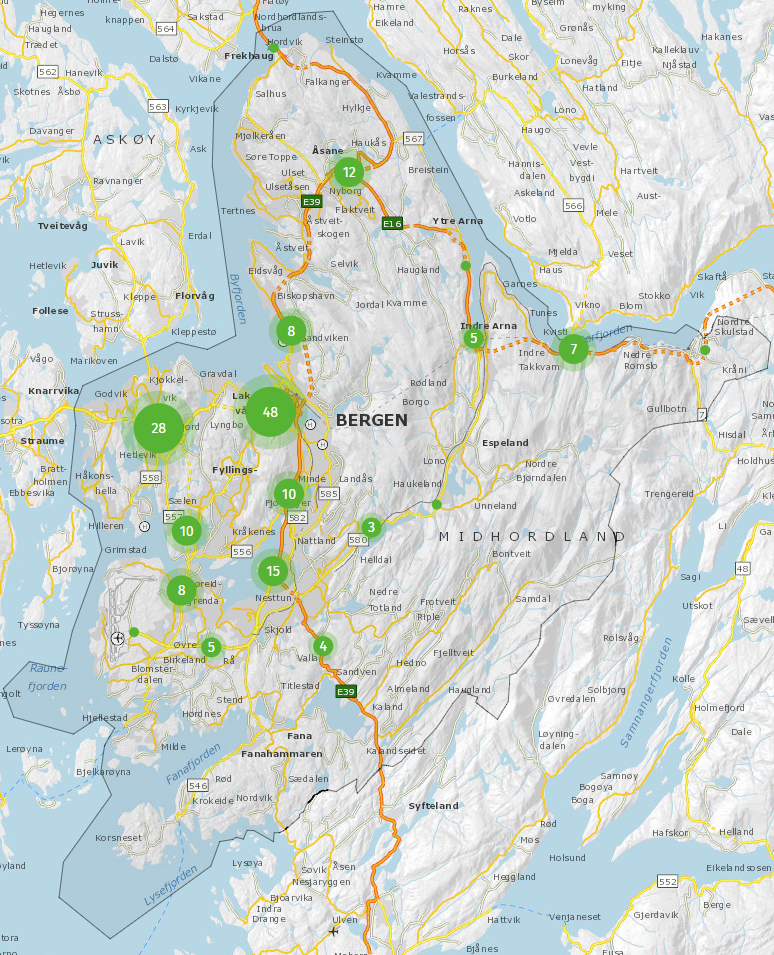
\includegraphics[width=16cm]{nivaa_1_bergen}
\centering
\caption{Geospatial bounds of Bergen}
\label{fig:boundsbergen}
\end{figure}

\begin{figure}[ht]
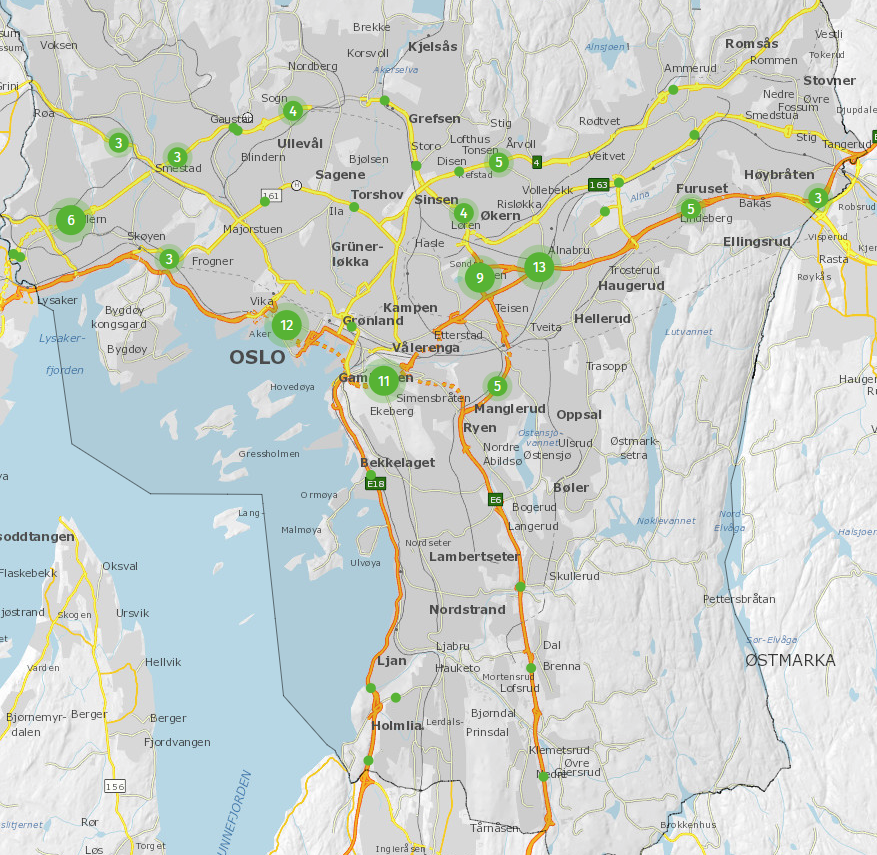
\includegraphics[width=16cm]{nivaa_1_oslo}
\centering
\caption{Geospatial bounds of Oslo}
\label{fig:boundsoslo}
\end{figure}

\begin{figure}[ht]
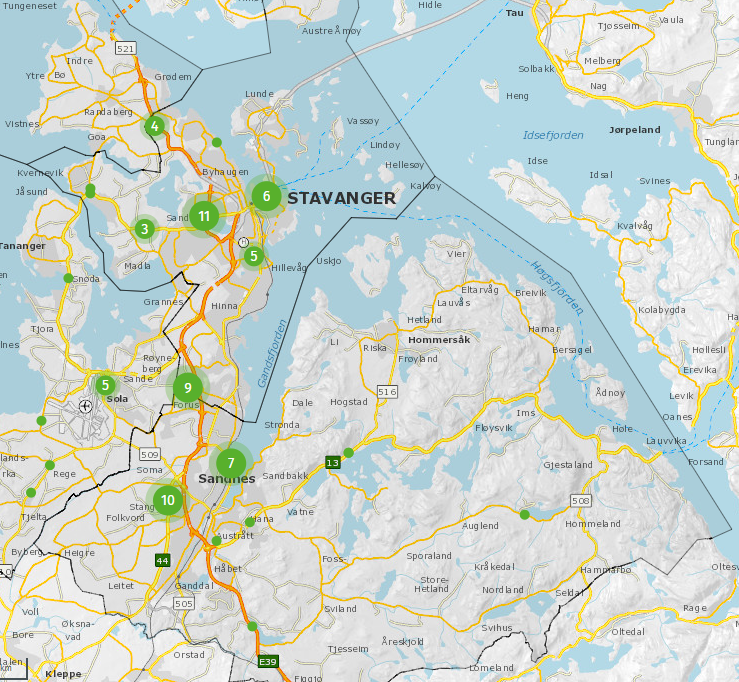
\includegraphics[width=16cm]{nivaa_1_stavanger}
\centering
\caption{Geospatial bounds of Stavanger}
\label{fig:boundsstavanger}
\end{figure}

The last NPRA dataset acquired was raw hourly data from a defined subset of all of NPRA's traffic registration stations previously used. The data contains all whole hours from all weeks over several years, number of fields available on the road (usually only two for regular roads), and how many vehicles passed by that hour and also their lengths in category. Figure \ref{fig:hboundsbergen}, \ref{fig:hboundsoslo} and \ref{fig:hboundsstavanger} shows the different geospatial hourly based bounds used. There are two modules dedicated to the hourly datasets, the NPRA\_Traffic\_Stations\_Graph.py and the NPRA\_Traffic\_Stations\_load\_data.py. The graph module is responsible for drawing a graph with specifications of hour to/from, weekday to/from, month to/from, year and field. The load data module is responsible for providing the graph with all the functions it needs to operate, like querying the dataset, the variance of the queried dataset, extracting the dataset from file and organizing it into a data structure, and reading and handling the coordinates of the traffic registration stations so that it can be shown on the map.

\begin{figure}[ht]
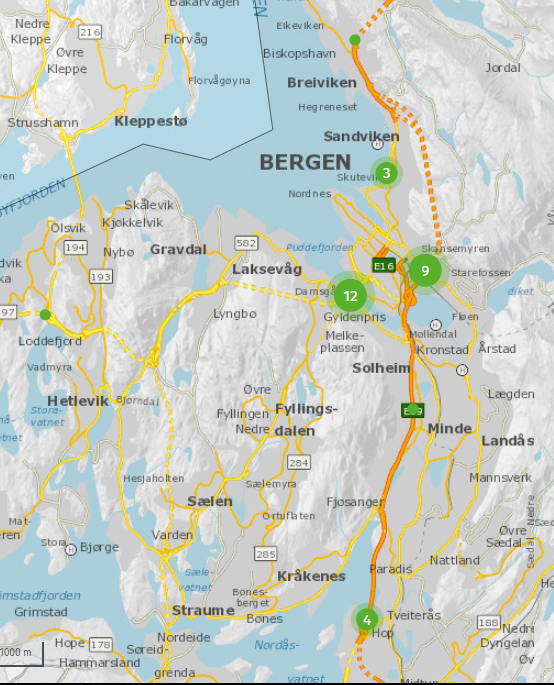
\includegraphics[width=16cm]{times_nivaa1_BERGEN}
\centering
\caption{Geospatial hourly bounds of Bergen}
\label{fig:hboundsbergen}
\end{figure}

\begin{figure}[ht]
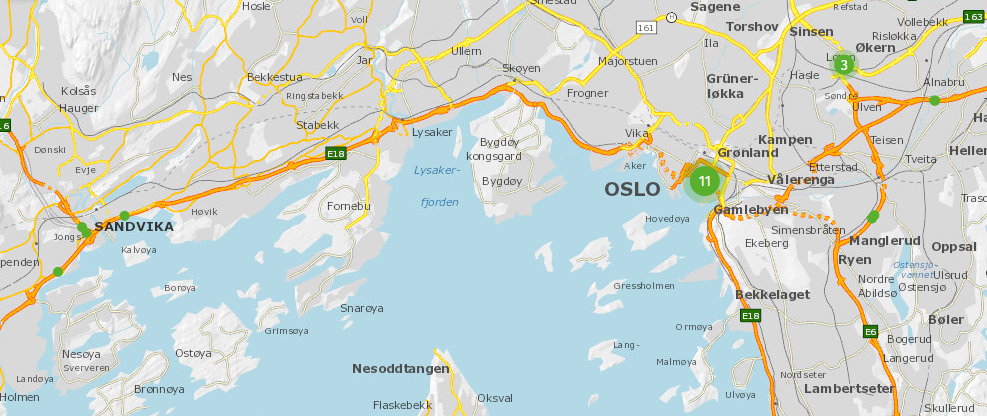
\includegraphics[width=16cm]{times_nivaa1_OSLO}
\centering
\caption{Geospatial hourly bounds of Oslo}
\label{fig:hboundsoslo}
\end{figure}

\begin{figure}[ht]
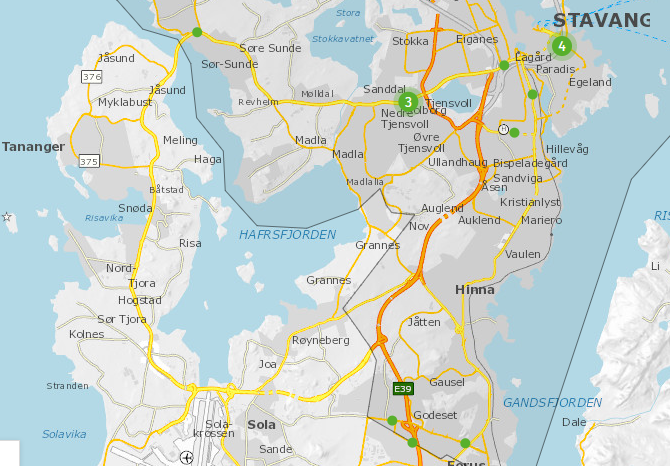
\includegraphics[width=16cm]{times_nivaa1_STAVANGER}
\centering
\caption{Geospatial hourly bounds of Stavanger}
\label{fig:hboundsstavanger}
\end{figure}

\newpage\newpage







\subsection{Twitter}
Using the representational state transfer (REST) application programming interface (API) it was paramount that in order to build a sufficient dataset acquiring and collecting data had to begin as soon as possible in order to collect enough data for this thesis. A simple python program was created that takes the input of the API keys provided by the file keys.txt and the keywords to be searched upon provided by the file search\_terms.txt. The program ensures that no duplicate messages are recorded, and the limit of a hundred tweets dictated by the REST API was overcome simply by searching for yet another hundred from the last date of the previous hundred until the date limit of about 10 days was reached.
The output is appended to a file in this data structure on new lines: id, date, location, tweet, there is also a dotted separator for each new tweet making it easy for humans to read. The functions described are implemented by the file twitter\_searching.py, which can be run as its own module and saves new tweets to the file twitter\_data.txt.

A straightforward analysis tool for the Twitter data in the file twitter\_data.txt was created by simply counting how many messages there are. The idea is that during influenza seasons numbers of tweets increases and then decrease when off the season. Figure \ref{fig:twitterAnal} shows the results. This function is implemented in the file twitter\_analyzer.py, when the module is executed on its own it shows a graph over the data found in the file twitter\_data.txt. A simple batch file twitter.bat was created to make it easy running these programs in the desired order.

\begin{figure}[ht]
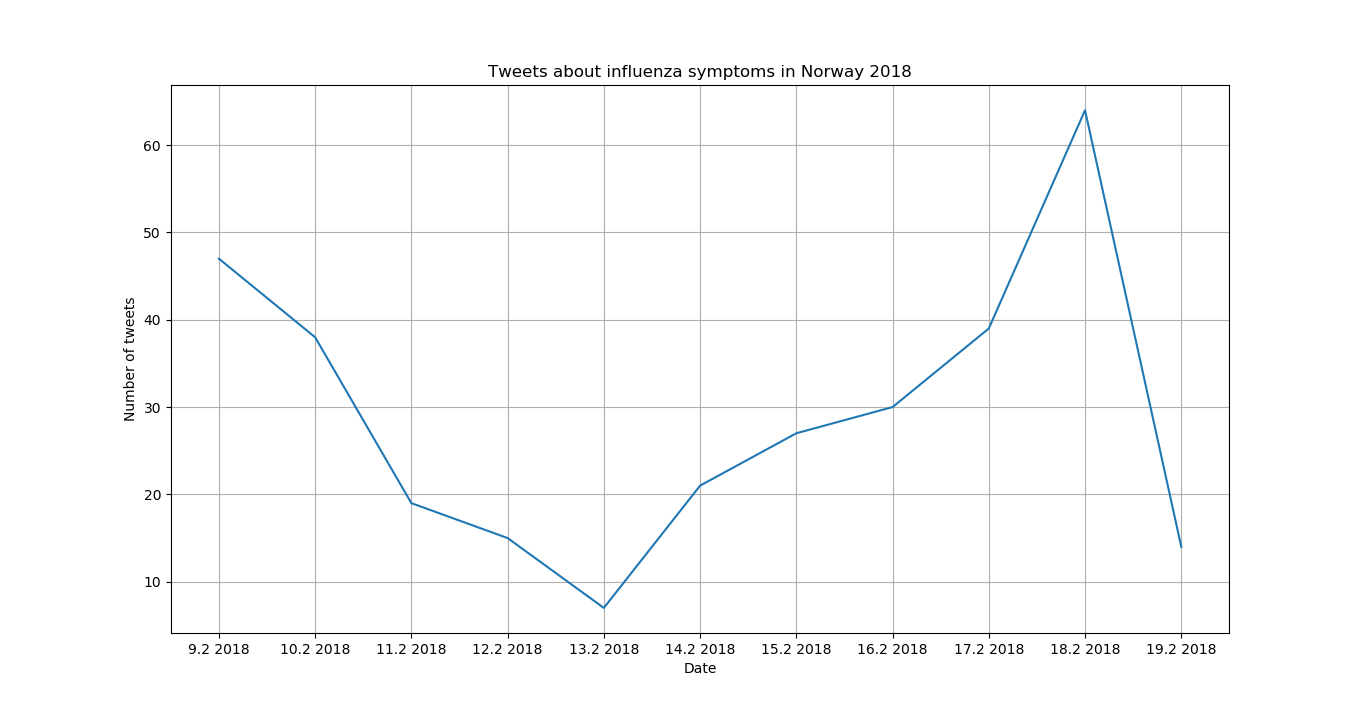
\includegraphics[width=16cm]{twitter_tweets_2018}
\centering
\caption{Tweets concerning ILS of 2018}
\label{fig:twitterAnal}
\end{figure}








\subsection{Kolumbus}
The data provided by Kolumbus was in a .png format and was converted into a more convenient comma separated values (CSV) file '15\_17\_månedstall\_total.csv'. From there it was a simple job to plot the data in a python script. Figure \ref{fig:kolumbus_15_17} shows the results.

\begin{figure}[ht]
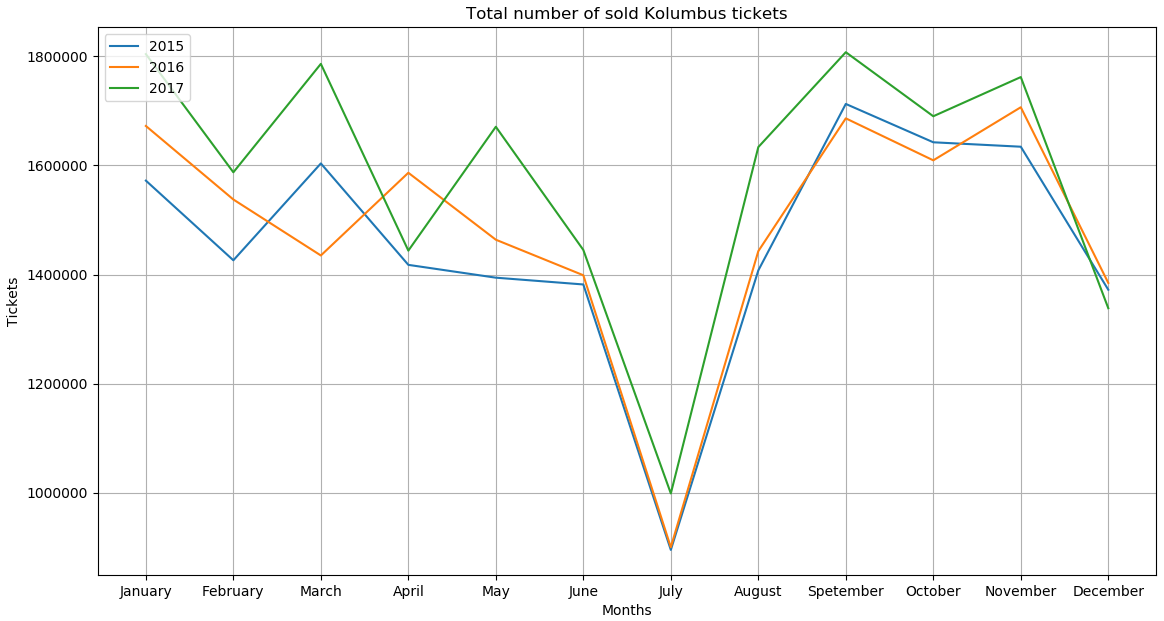
\includegraphics[width=16cm]{kolumbus_total_num_sold_15_17}
\centering
\caption{Monthly passenger travel with Kolumbus}
\label{fig:kolumbus_15_17}
\end{figure}









\subsection{Ruter}
The data provided by Ruter was in a .xlsx file and could easily be read, extracted and plotted by a simple python script. Figure \ref{fig:ruter_15_18} shows the results.

\begin{figure}[ht]
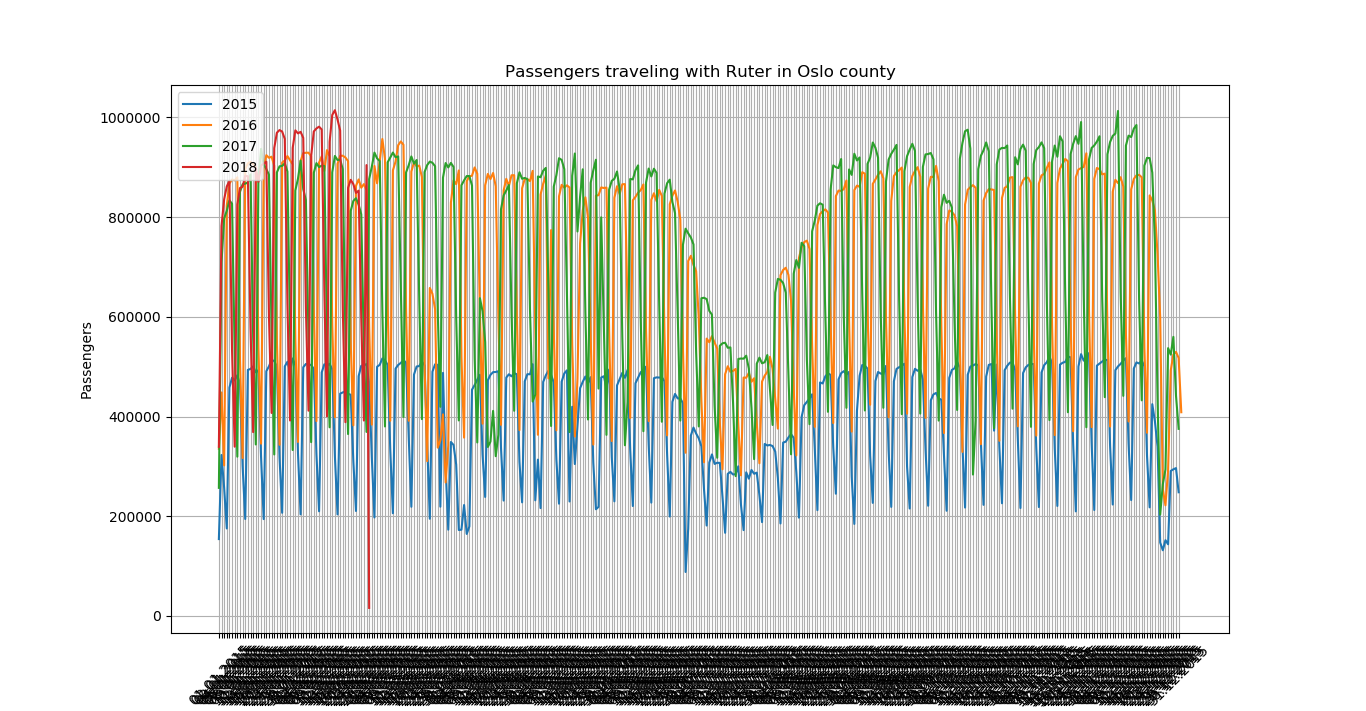
\includegraphics[width=16cm]{ruter_15_18}
\centering
\caption{Daily tickets sold with Ruter, the year of 2015 does not contain metro services}
\label{fig:ruter_15_18}
\end{figure}










\section{The Frontend}
The thesis is divided into two: The backend and the frontend. The frontend is responsible for visualizing a representation of the data provided by the backend. It does so by mounting a graphical user interface (GUI) that provides everything the user needs from this thesis. The GUI uses other frontend modules described in the following subchapters.

\subsection{The GUI}
The file gui.py is the main program. It serves the GUI with help from the backend, the file map\_canvas.py, and the file scrframe.py. The GUI is created using Python's standard Tkinter module, and it provides the mean of a window creation with all the usual GUI interface needs available. 

The GUI is structured in two parts: The buttons frame and the data frame. The buttons frame simply makes available buttons to be clicked upon showing the different graphs for the respective datasets from the backend. The data frames show the graphs and if needed a map, visualizing the data from the backend. The backend takes time to load, to make this experience more user-friendly a progress bar is shown progressing in real time relative to the loading sequence. Upon completion, the NPIH data is shown as a standard view. The user may use the mouse wheel to scroll up and down the view and click the buttons to change datasets. 

In some datasets, a map is provided for further visualization. the map is interactive with its own button and also responds to dragging the mouse in order to move the map, double-clicking in order to zoom in and using the mouse wheel to zoom in and out.

\subsection{The Map}
The file map\_canvas.py provides the GUI a Goompy\cite{goompy} map. This file is also from the Goompy project, but is heavily modified to serve the purpose of this thesis. The file launches a Google static API map on a Tkinter canvas and provides basic functions like user input. The functions edited by the author of the thesis is: better zooming capabilities, coordinate markers, ability to focus on the map by will and some minor bug fixes.

\subsubsection{Goompy}
Goompy\cite{goompy} provides an interactive Google static map for Python and is created by Simon D. Levy.
The core Goompy file is found in the file /Frontend/goompy/\_\_init\_\_.py. This was heavily edited to provide the necessary functions of this thesis. The edit includes: Multithreading the fetching of Google static map images, making Goompy about 4 times faster, dragging now changes latitude and longitude to better help zooming functions, having the API key fetched from a separate text file such to hide this from misuse by other developers, supporting map coordinates to be plotted directly in the google static API, drawing the coordinates with polygon and colors and using the mouse wheel to zoom in and out. Goompy requires a Google static map API key in order to work properly, users are asked to create a file Frontend/api\_keys.txt and paste the key there as described by the file Frontend/README.md.

\subsection{The Scrollbar}
Creating a functional scrollbar that responds to mouse click and mouse wheel events in Tkinter proved difficult, which is why Eugene Bakin's Tkinter scollable\cite{scrframe} frame was used. The file Frontend/scrframe.py contains his code with minor edits in order to be able to scroll with the mouse wheel, get the Tkinter focus, resetting scrollbar viewport and better resizing of the window. This module may also be run independently for testing purposes.





